% ****** Start of file apssamp.tex ******
%
%   This file is part of the APS files in the REVTeX 4.1 distribution.
%   Version 4.1r of REVTeX, August 2010
%
%   Copyright (c) 2009, 2010 The American Physical Society.
%
%   See the REVTeX 4 README file for restrictions and more information.
%
% TeX'ing this file requires that you have AMS-LaTeX 2.0 installed
% as well as the rest of the prerequisites for REVTeX 4.1
%
% See the REVTeX 4 README file
% It also requires running BibTeX. The commands are as follows:
%
%  1)  latex apssamp.tex
%  2)  bibtex apssamp
%  3)  latex apssamp.tex
%  4)  latex apssamp.tex
%
\documentclass[%
 reprint,
%superscriptaddress,
%groupedaddress,
%unsortedaddress,
%runinaddress,
%frontmatterverbose,
%preprint,
%showpacs,preprintnumbers,
%nofootinbib,
%nobibnotes,
%bibnotes,
amsmath,amssymb,
%aps,
pra,
%prb,
%rmp,
%prstab,
%prstper,
%floatfix,
]{revtex4-1}

\usepackage{siunitx}
\usepackage{graphicx}% Include figure files
\usepackage{dcolumn}% Align table columns on decimal point
\usepackage{bm}% bold math
%\usepackage{hyperref}% add hypertext capabilities
%\usepackage[mathlines]{lineno}% Enable numbering of text and display math
%\linenumbers\relax % Commence numbering lines

%\usepackage[showframe,%Uncomment any one of the following lines to test
%%scale=0.7, marginratio={1:1, 2:3}, ignoreall,% default settings
%%text={7in,10in},centering,
%%margin=1.5in,
%%total={6.5in,8.75in}, top=1.2in, left=0.9in, includefoot,
%%height=10in,a5paper,hmargin={3cm,0.8in},
%]{geometry}

\begin{document}

\preprint{APS/123-QED}

\title{Fabrication and characterization of a Pseudo-MOSFET}% Force line breaks with \\

\author{Moritz Berger}
 \altaffiliation[]{RWTH Aachen University, Germany}%Lines break automatically or can be forced with \\
 \email{moritz.berger@rwth-aachen.de}
 \author{Gerald Kolter}
 \altaffiliation[]{RWTH Aachen University, Germany}%Lines break automatically or can be forced with \\
 \email{gerald.kolter@rwth-aachen.de}

\date{\today}% It is always \today, today,
             %  but any date may be explicitly specified

\begin{abstract}
bla
\end{abstract}

\maketitle

\section{Introduction}
In the following the fabrication of a Pseudo-MOSFET ("metallic-oxide-semiconductor-field-effect-transistor") will be described. The next step is a more detailed description of optical lithographie and reactive ion etching. Afterwards an analysis and a discussion of the characterization of the fabricated Pseudo-MOSFET will be given.

\section{Fabrication}

\begin{table}
\centering
\begin{tabular}{|c|c|}
\hline 
Fabrication technology & "UNIBOND" \\ 
\hline 
top Si thickness & \SI{85}{nm} \\ 
\hline 
buried oxide thickness & \SI{145}{nm} \\ 
\hline 
doping type & p-type (Boron) \\ 
\hline 
doping concentration & $1 \times 10^{15}$ \si{\per\cubic\centi\meter} \\ 
\hline 
crystal orientation & (100) \\ 
\hline 
\end{tabular} 
\caption{Specification of the SOI wafer.}
\label{tab:Spec_SOI}
\end{table}

The basis for the MOSFET are SOI (Semiconductor On Insulator) samples, the specifications are listed in table \ref{tab:Spec_SOI}. Si is used as semiconductor and SiO$_2$ as insulator. In a first step an mask for the following etching was defined lithographically. The mesa structuring is done by reactive ion etching with a gas mixture of SF$_6$/O$_2$. For removing the resist an oxygen plasma is used. At next the samples are RCA-cleaned ending with a dip in hydroflourid acid to get a bare silicon surface. The aluminum is deposited in a vacuum. The aluminum layer is structured with optical lithographie and an aluminum etching as which phosphoric acid, nitric acid, acetic acid and water in a volume ratio of 16:1:1:2 is used. 

\section{Theory}
\subsection{Optical Lithographie}

\subsection{Reactive Ion Etching}
\section{Measurement}
\section{Data Analysis}
In the following chapter the characteristic values of the MOSFETs are extracted out of the measurement data. The methods that are used to do this are shown with the help of the data set of device A5 of the lower right quadrant (4-A5). This device has a tunnel length of \SI{200}{\mu m} with an inner radius of \SI{25}{\mu m} and an outer radius of \SI{225}{\mu m}.
\subsection{Output Characteristics}
\begin{figure}
\centering
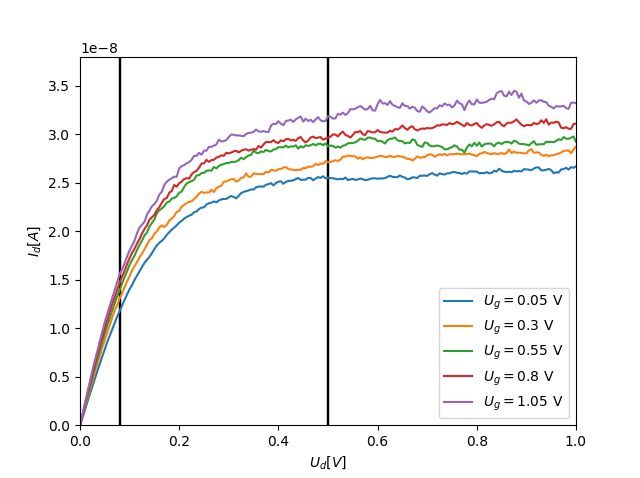
\includegraphics[scale=0.6]{Bilder/output.png}
\caption{Output curves for different gate-voltages.}
\label{fig:output}
\end{figure}

The output characteristics of one device was measured to determine an appropriate gate voltage. As predicted by theoretical calculations the curves show a linear behavior for small drain-voltages. For the measured device and gate-voltages this goes up to approximately $U_d \approx \SI{0.08}{V}$. They enter saturation at around $U_d \approx \SI{0.5}{V}$. As a result of this three drain-voltages in the linear regime ($U_d = \SI{0.3}{V},\SI{0.5}{V} $ and \SI{0.7}{V}) were chosen and the transfer-characteristic was measured for each of these values.

\subsection{Transfer Characteristic}
\subsubsection{Effective Carrier Charge Density}
For the extraction of the effective carrier charge density $\mu_{eff}$ the $\dfrac{I_d}{\sqrt{g_m}}$-method is used.\\
\\
In a first step the measured drain-current $I_d$ is plotted against the gate-voltage $V_g$ for three different drain-voltages $V_d$ = \SI{0.03}{V}, \SI{0.05}{V} and \SI{0.07}{V} , as seen in figure \ref{fig:linreg1}. Then the point with the highest slope is determined numerically and a linear regression is fitted at a \SI{1}{\volt} area around this point. The resulting straights are also shown in figure \ref{fig:linreg1}.
\begin{figure}
\centering
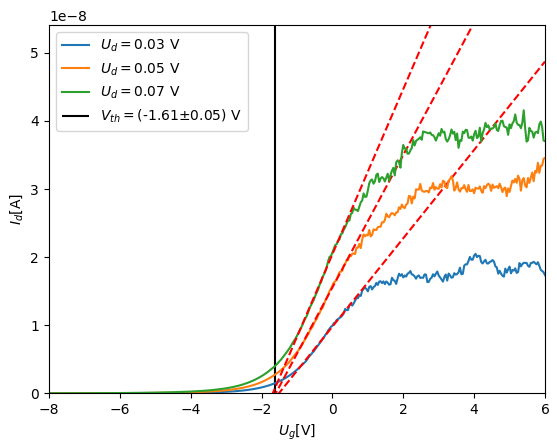
\includegraphics[scale=0.6]{Bilder/linreg.png}
\caption{drain-current $I_d$ plotted against the gate-voltage $V_g$ for different drain Voltages.}
\label{fig:linreg1}
\end{figure}

The threshold-voltage $V_{th}$, as well as its error, can directly be extracted from this fit. This is done for all three curves and a final value for $V_{th}$ for this device is calculated by taking the weighted average of all three values.\\
\\
The slope of this fit is also used to determine $\mu_{eff}$ with the help of the following equation:
\begin{equation}
\sqrt{\mu_{eff} f C_{ox} V_d} \cdot (V_g-V_{th}) = \dfrac{I_d}{\sqrt{g}}
\end{equation}

where $f = 2\pi / ln(R_2/R_1)$ is a structural factor, $C_{ox} = \epsilon_0 \epsilon_{ox} / d_{ox}$ is the capacity of the oxide-layer and g is the slope. $\epsilon_{ox} = 3.9$ is used. A constant error of \SI{0.1}{\mu m} is assumed for the radii $R_1$ and $R_2$ to account for uncertainties in the fabrication process.\\
In order to determine  $\mu_{eff}$ the right side of this equation $I_d/\sqrt{g}$ is plotted against $V_g$, as seen in figure \ref{fig:linreg2}. This figure displays $I_d/\sqrt{g}$ plotted against $V_g \cdot \sqrt{V_d}$ in order to compare the tree slopes without the differing influence of $V_d$. A second linear regression is then fitted to the data. From the slope $a$ of this fit one can get $\mu_{eff}$ through the following equation:
\begin{equation}
\mu_{eff} = \dfrac{a^2}{f C V_d}
\end{equation}
This is also done for all three drain-voltages. A final value for $\mu_{eff}$ is again calculated by taking the weighted average. The results are listed in table \ref{tab: exaple_data}.

\begin{table}
\centering
\begin{tabular}{|c|c|c|c|}
\hline
$U_d$ & $V_{th}[\si{V}]$ & $g[\si{nA/V}]$ & $mu_{eff}[\si{cm^2/Vs}]$\\
\hline
0.03 & $-1.51\pm 0.02$ & $6.48\pm 0.07$ & $0.59\pm 0.02$\\
\hline
0.05 & $-1.6\pm 0.02$ & $9.72\pm 0.09$ & $0.53\pm 0.01$\\
\hline
0.07 & $-1.69\pm 0.02$ & $12.12\pm 0.1$ & $0.47\pm 0.01$\\
\hline
average & $-1.61\pm 0.05$ & $8.64\pm 1.6$ &$0.51\pm 0.03$\\
\hline
\end{tabular}
\label{tab: exaple_data}
\caption{Results for device 4-A5.}
\end{table}



\begin{figure}
\centering
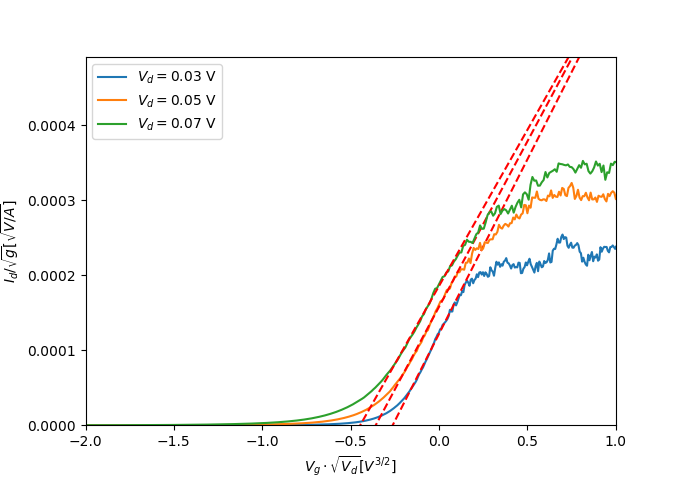
\includegraphics[scale=0.6]{Bilder/mu.png}
\caption{$I_d/\sqrt{g}$ plotted against $V_g \cdot \sqrt{V_d}$ for different drain Voltages.}
\label{fig:linreg2}
\end{figure}

\subsubsection{subthreshold-slope}

\begin{figure}
\centering
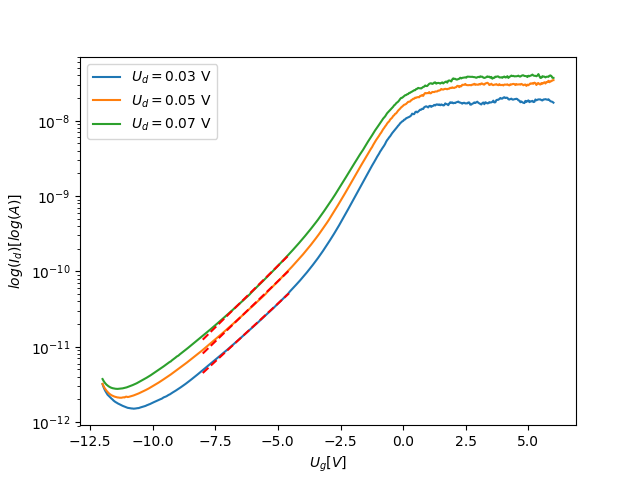
\includegraphics[scale=0.6]{Bilder/log.png}
\caption{$log(I_d)$ plotted against $V_g$ for different drain Voltages to analyze the subthreshold slope.}
\label{fig:log}
\end{figure}

The subthreshold slope is an important characteristic of a Mosfet because it gives an indication for how fast it can change its behavior. A steeper slope means that a smaller voltage difference is required for it to be turned on, which can be achieved quicker. A perfect Mosfet would have a step-fuction slope.\\
\\
In order to analyze the subthreshold slope the drain-current is plotted logarithmicly against the gate-voltage as shown in figure \ref{fig:log}. A voltage area is then manually  selected, in which the curves appear to be linear. In this area a linear fit is fitted against the curves in order to obtain the slope. Because the subthreshold slope is usually given by the unit $\si{V/dec}$ the final value is obtained by
\begin{equation}
\Delta U = \dfrac{log(10)}{a}
\end{equation}
where $a$ denotes the initial slope.\\
For the example device the voltage for the fit ranges from \SI{-8}{V} to \SI{-4.5}{V}. The results of this are shown in table \ref{tab:subthreshold_example}.

\begin{table}
\centering
\begin{tabular}{|c|c|c|}
\hline
$U_d$[\si{V}] & a [log(A)/V] & subthreshold-slope [V/dec] \\
\hline
0.03 & $0.71\pm 0.02$ & $3.26\pm 0.10$\\
\hline
0.05 & $0.74\pm 0.03$ & $3.13\pm 0.11$\\
\hline
0.07 & $0.75\pm 0.03$ & $3.06\pm 0.11$\\
\hline
average & $0.73\pm 0.02$ & $3.16\pm 0.09$\\
\hline
\end{tabular}
\label{tab:subthreshold_example}
\caption{Results of the subthreshold analysis.}
\end{table}

\subsubsection{Ambipolarity}
The curve that was analyzed until now shows a current flow for increasing gate-voltages. This corresponds to electrons moving through the device. However for certain devices there also exists a current flow for decreasing gate-voltages, as shown in figure \ref{fig:ambipol} for device 4-C3. This can be explained by the fact that (positively charged) electron-holes can move through the device for negative gate-voltages. This phenomenon is called Ambipolarity

\begin{figure}
\centering
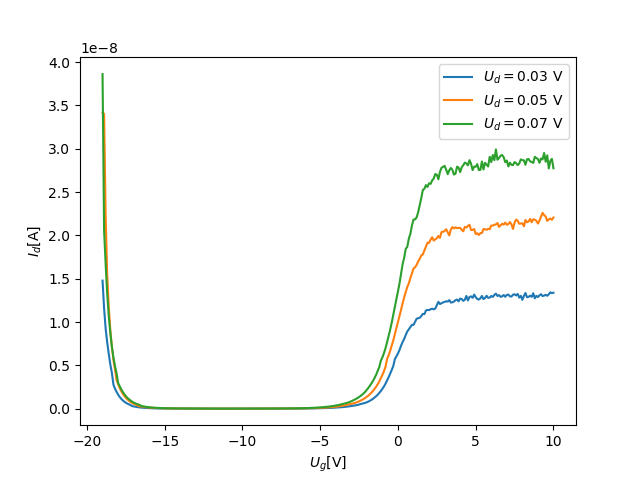
\includegraphics[scale=0.6]{Bilder/amipol.png}
\caption{transfer characteristic of device 4-C3 for the full negative range of $V_g$. A second current flow can be observed for large negative voltages.}
\label{fig:ambipol}
\end{figure}


\section{Results and Discussion}
The Analysis described in the previous chapter is done for all measured devices. The results are listed in table \ref{tab:transfer_results}.\\
\\



\begin{table}
\centering
\begin{tabular}{|c|c|c|c|c|c|c|}
\hline 
Position & length & $R_1$ & $R_2$ & $V_{th}$ [\si{\volt}]  & $\mu_{eff}$  [\si{cm^2/Vs}] & subthreshold \\ 
\hline 
4a1 & 50 & 25 & 75 & $-2.63\pm 0.14$ & $0.21\pm 0.03$ & $1.93\pm 0.07$\\
\hline 
3d1 & 50 & 50 & 100 & $-1.28\pm 0.01$ & $5.09\pm 0.07$& $2.1\pm 0.11$\\
\hline 
3e1 & 50 & 150 & 200 & $-0.61\pm 0.01$ & $4.27\pm 0.01$& $3.07\pm 0.09$\\
\hline 
\hline 
1b2 & 75 & 50 & 125 & $-0.54\pm 0.02$ & $7.62\pm 0.22$& $2.68\pm 0.1$\\
\hline 
1d2 & 75 & 100 & 175 & $-4.29\pm 0.35$ & $0.07\pm 0.01$& $3.33\pm 0.05$\\
\hline 
4e2 & 75 & 150 & 225 & $1.31\pm 0.17$ & $0.57\pm 0.04$& $6.28\pm 0.32$\\
\hline 
\hline  
4b3 & 100 & 50 & 150 & $-4.03\pm 0.05$ & $0.08\pm 0.01$& $3.06\pm 0.05$\\
\hline 
4c3 & 100 & 75 & 175 & $-1.51\pm 0.01$ & $0.72\pm 0.02$& $2.65\pm 0.13$\\
\hline 
4e3 & 100 & 150 & 250 & $-3.41\pm 2.08$ & $0.04\pm 0.01$& $8.85\pm 0.18$\\
\hline
\hline 
4b4 & 150 & 50 & 200 & $-4.9\pm 0.24$ & $0.04\pm 0.01$& $3.22\pm 0.05$\\
\hline
4c4 & 150 & 75 & 225 & $0.25\pm 0.01$ & $3.0\pm 0.08$& $4.22\pm 0.22$\\
\hline 
4d4 & 150 & 100 & 250 & $-4.08\pm 0.08$ & $0.13\pm 0.01$& $3.16\pm 0.05$\\
\hline 
4e4 & 150 & 150 & 300 & $-5.34\pm 1.73$ & $0.04\pm 0.01$& $10.76\pm 0.39$\\
\hline 
\hline 
4a5 & 200 & 25 & 225 & $-1.61\pm 0.05$ & $2.77\pm 0.17$& $3.16\pm 0.09$\\
\hline 
4b5 & 200 & 50 & 250 & $-2.34\pm 0.02$ & $0.85\pm 0.03$& $3.04\pm 0.05$\\
\hline 
4c5 & 200 & 75 & 275 & $-3.19\pm 0.22$ & $0.09\pm 0.02$& $4.72\pm 0.28$\\
\hline
4d5 & 200 & 100 & 300 & $-1.21\pm 0.02$ & $2.65\pm 0.03$& $2.8\pm 0.03$\\
\hline 
4e5 & 200 & 150 & 350 & $-1.56\pm 0.06$ & $1.79\pm 0.1$& $2.69\pm 0.05$\\
\hline 
\end{tabular} 
\caption{Results of transfer characterization.}
\label{tab:transfer_results}
\end{table}

\subsection{further analysis}





\section{Conclusion}

\bibliography{MOSFET}% Produces the bibliography via BibTeX.

\end{document}

\begin{thebibliography}{x}
   \bibitem[Esselborn-Krumbiegel, H., 2008]{bmbf} Von der Idee zum Text. Eine Anleitung zum wissenschaftlichen Schreiben. Paderborn: Verlag Ferdinand Sch�ningh GmbH \& Co. KG.

   \bibitem[Franck, N., 2004]{bmbf} Handbuch Wissenschafliches Arbeiten. Frankfurt am Main: Fischer Taschenbuch Verlag.
Karmasin, M., \& Ribing, R. (2011). Die Gestaltung wissenschaftlicher Arbeiten. Wien: Facultas Verlags- und Buchhandels AG.

   \bibitem[Lengauer, H., \& Wimmer, A., 2006]{bmbf} http://www.uni-klu.ac.at. Abgerufen am 30. 9. 2013 von Definition Plagiat: http://www.uni-klu.ac.at/main/inhalt/3054.htm

   \bibitem[Prei�ner, A., 2012]{bmbf} Wissenschaftliches Arbeiten: Internet nutzen, Text erstellen, �berblick behalten. M�nchen: Oldenbourg.

\end{thebibliography}
